% Modern Aspect Ratio
\documentclass[aspectratio=169]{beamer}

% Set theme
\usetheme{metropolis}

% Remove navigation symbols
\setbeamertemplate{navigation symbols}{}

% Fonts
\usefonttheme[onlymath]{serif}
% \usepackage[scaled]{helvet}

% Plots
\usepackage{pgfplots}

% Math
\usepackage{mathrsfs}

% QR Code
\usepackage{qrcode}


\title{Metrics for Responsible AI Projects}
\subtitle{Data Intelligence Tokyo Meetup}
\author{Victor Steinborn}
\date{September 30, 2025}

\begin{document}

\frame{\titlepage}

\begin{frame}{About me}
	\begin{itemize}
		\item PhD in computer science
		      \begin{itemize}
			      \item LMU Munich, Germany
			      \item Research focus: Responsible AI
		      \end{itemize}
		\item Industry Experience: Responsible AI Research and Software Development
	\end{itemize}
\end{frame}

\section{Responsible AI}

\begin{frame}{What is Responsible AI?}
	\begin{itemize}
		\item Study of developing and deploying AI systems responsibly
		\item Some topics:
		      \begin{itemize}
			      \item Fairness
			      \item Alignment
			      \item Explainability
			      \item Environment
		      \end{itemize}
	\end{itemize}
\end{frame}

\begin{frame}{Why Responsible AI?}
	\begin{itemize}
		\item An opportunity to think about social and environmental impact
		\item Framework to align metrics to (unforeseen) project constraints
	\end{itemize}
\end{frame}

\section{ChatGPT Case Study}

\begin{frame}{ChatGPT (Recap)}
	\begin{itemize}
		\item ChatGPT first released November 2022 with GPT-3.5 \cite{openai_introducing_2022}
		\item Focus on the predecessor model, GPT-3 \cite{brown_language_2020}
	\end{itemize}
\end{frame}

\begin{frame}{GPT-3 Model Training \cite{brown_language_2020}}
	\begin{center}
		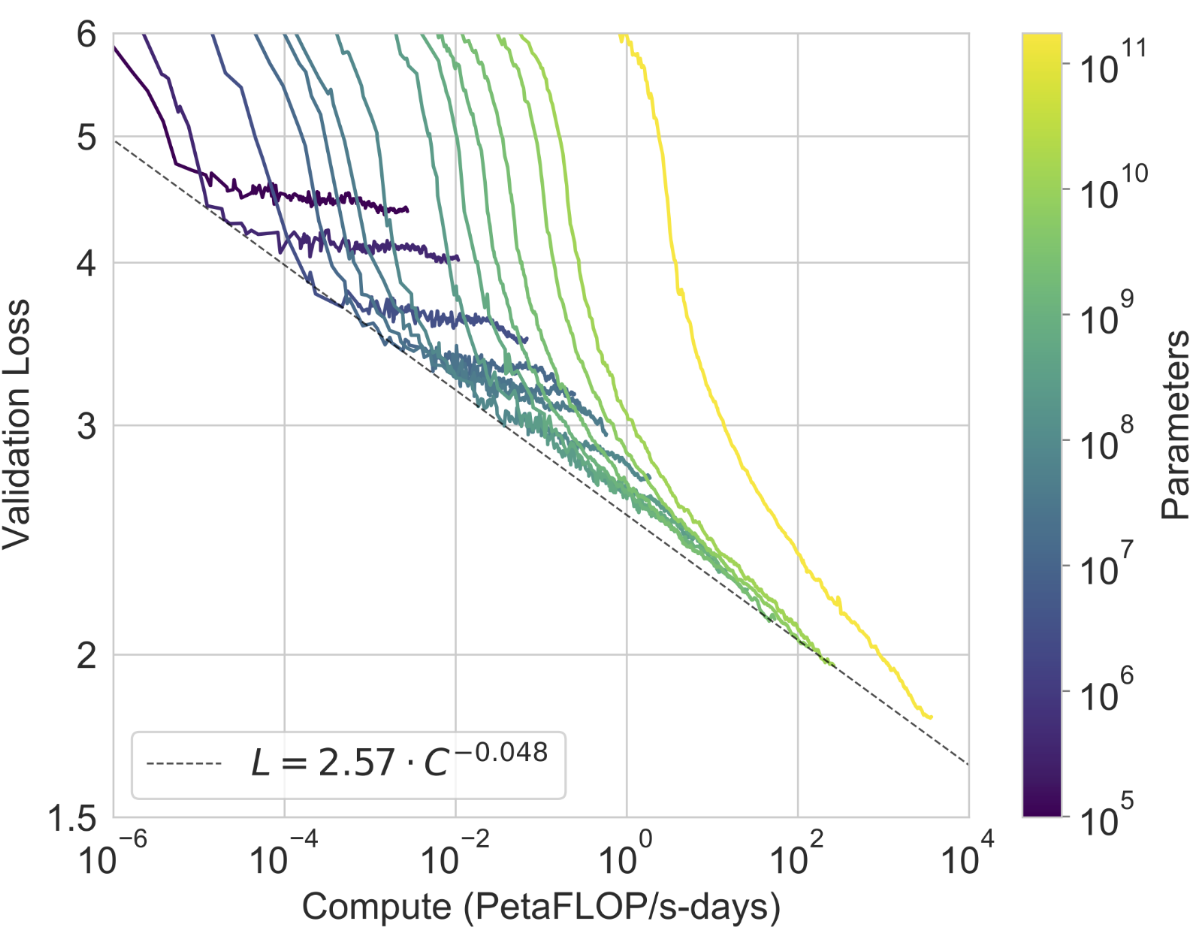
\includegraphics[width=0.6\textwidth]{images/gpt3-training.png} \\
		$\uparrow$ Parameters $\rightarrow$ $\downarrow$ Loss ($\uparrow$ Training Performance) AND $\uparrow$ Compute
	\end{center}
\end{frame}

\begin{frame}{Power}
	Definition of Power:
	\begin{equation*}
		\mathscr{P} = \frac{dE}{dt}
	\end{equation*}
	\begin{itemize}
		\item Training GPT-3 consumes about 1.287 \emph{GWh} of energy \cite{luccioni_estimating_2022}
		\item 1GWh is a huge amount of energy
	\end{itemize}
\end{frame}

\begin{frame}{How Much is 1 GWh? \cite{usde_how_2024}}
	\begin{center}
		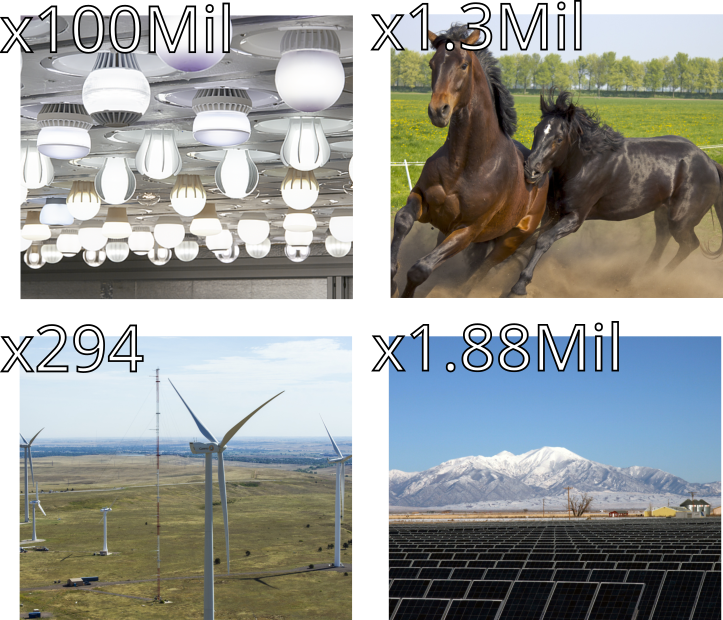
\includegraphics[width=0.5\textwidth]{images/onegw.png} \\
		For 1 Hour
	\end{center}
\end{frame}

\begin{frame}{Energy Consumption in AI Today \cite{zoe_schiffer_openai_2025}}
	\begin{center}
		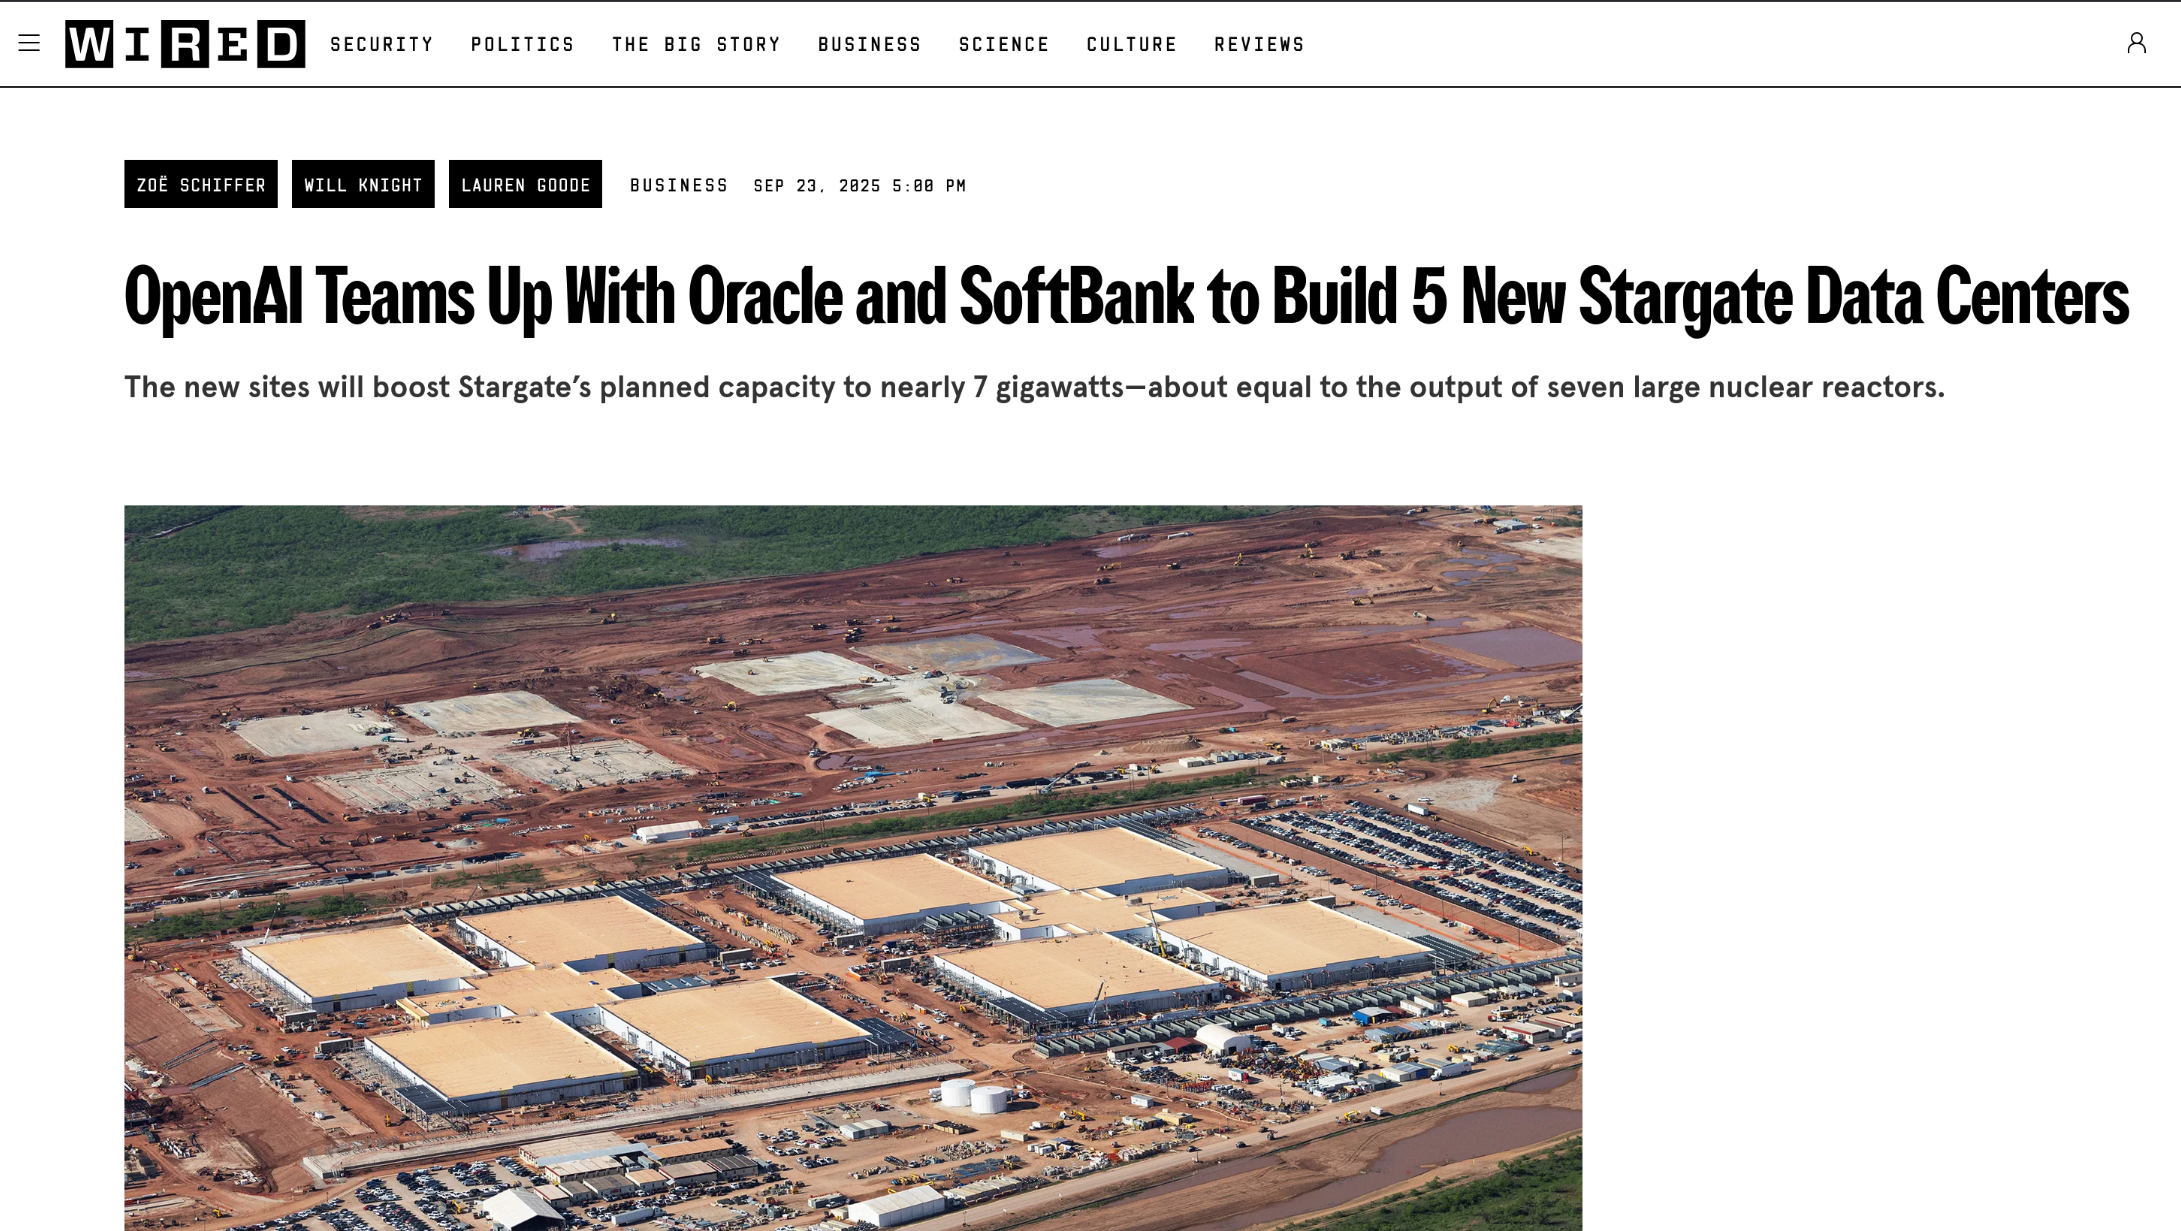
\includegraphics[width=0.8\textwidth]{images/wired-article.png}
	\end{center}
\end{frame}

\section{What We Can Do}

\begin{frame}{Guidelines \cite{united_nations_united_2015}}
	\begin{center}
		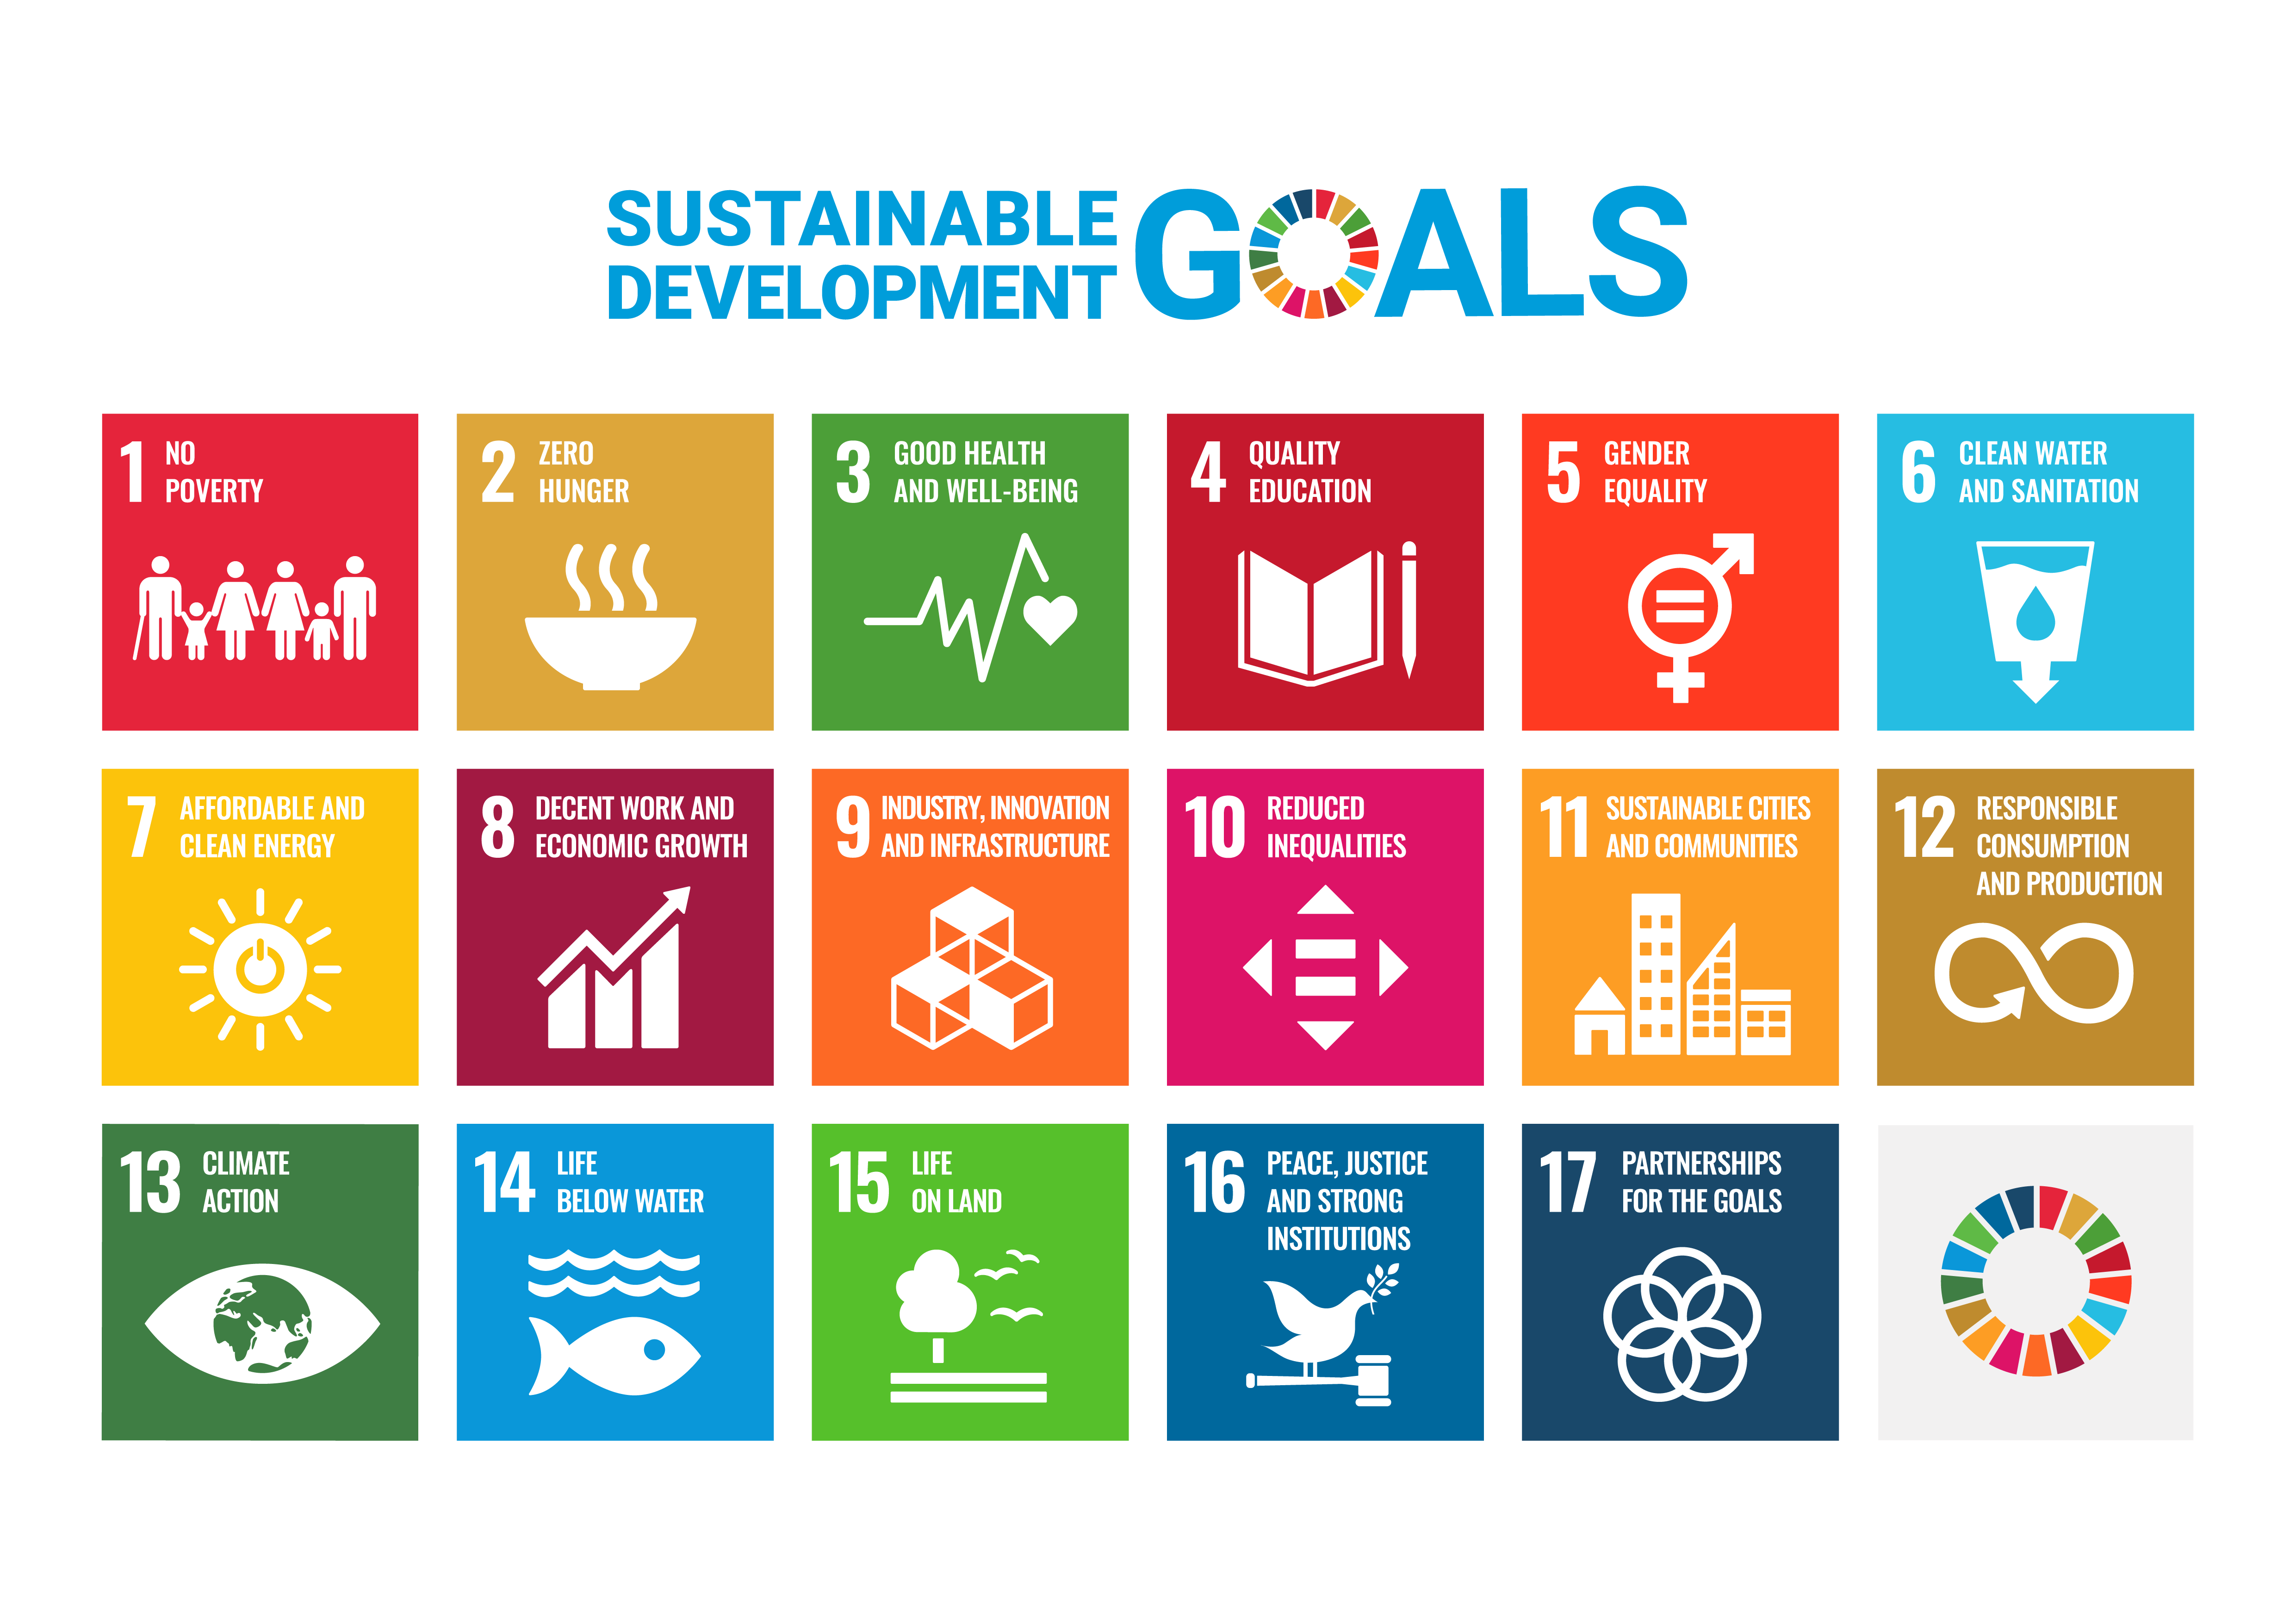
\includegraphics[width=0.8\textwidth]{images/E_SDG_poster_WEB.png}
	\end{center}
\end{frame}

\begin{frame}[standout]
	Questions?
\end{frame}

\begin{frame}[allowframebreaks]{References}

	\bibliography{2025-09-30-RAImetrics}
	\bibliographystyle{abbrv}

\end{frame}

\end{document}
